%\documentclass{cumcmthesis}
\documentclass[withoutpreface,bwprint]{cumcmthesis} %去掉封面与编号页
%\usepackage{graphicx}
%\usepackage{subfigure}
\usepackage{tabularx}
\title{论文题目}
\tihao{C}            % 题号
\baominghao{202217241200}    % 报名号
\schoolname{华中科技大学}
\membera{卢凯}
\memberb{陈铭锐}
\memberc{房怿宽}
\supervisor{胡勇}
\yearinput{2022}     % 年
\monthinput{09}      % 月
\dayinput{15}        % 日

\begin{document}
	\maketitle
	\begin{abstract}
		摘要的具体内容。
		\keywords{关键词1\quad  关键词2\quad   关键词3}
	\end{abstract}
	%\tableofcontents
	
	
%----------- 正文 ----------
%----------- 一、问题重述 ----------
		\section{问题重述}
		\subsection{问题背景}
		\par 无人机是“无人驾驶空中飞行器”(UAV)的简称。1917年首先由英国研制出来最先承担起军事功能,诸如目标定位跟踪技术在航空、航天和航海领域都有十分重要的地位。无源定位技术是被动工作方式的目标定位技术,利用未知目标的辐射源信号进行定位和导航。
		\subsection{待求解的问题}
		\par 
		\begin{enumerate}
			\item{\textbf{问题一中第一问}:}在已知三架编号已知、位置无偏差的无人机且其中一架为位于圆心的无人机FY$ 00 $为承担发射信号任务的无人机的既定条件下,根据圆周上其他的位置存在偏差的无人机被动接受的方向信号建立模型来完成对该被动接收信号无人机的纯方位无源定位。
			\item{\textbf{问题一中第二问}:}在编队方式仍为圆周,且无人机数目仍为10架的相同条件下,修改发射信号的无人机为编号FY$ 00 $和FY$ 01 $的无人机与待定数量未知编号的无人机。发射信号的无人机的位置没有偏差,确定除了已知编号的无人机FY$ 00 $和无人机FY$ 01 $外,最少需要几架未知编号的无人机作为位置无偏差的无人机来发射信号以期望实现无人机的有效定位。
			\item{\textbf{问题一中第三问}:}在编队方式与无人机数目基础条件均不变的基础上,设定无人机所处圆周的半径为100m。初始时刻无人机的位置确定但略有偏差,试确定在编号为FY$ 00 $的无人机和圆周上数量不超过三架的无人机作为发射信号的无人机的条件下,忽略每次调整的时间,调整到理想位置使九架无人机均匀的分布在某个圆周上的最优调整方案。
			\item{\textbf{问题二}:}
		\end{enumerate}
%----------- 二、问题分析 ----------
	\section{问题分析}
		\subsection{问题一:}
		在第一题的大背景下,我们可以知道,无人机的数目和编队的方式,并且给定的条件为有三架已知编号且位置没有误差的无人机作为发射信号的无人机。我们需要根据其余位置有偏差的无人机被动接受到的方位信号即三个角度信息从而实现定位。
		\subsection{问题二:}
		在问题二中,我们首先假设对于任意的$D_i$,通过测量$D_0,D_1,D_j$三个无人机的位置,得到两个小角$\alpha_1,\alpha_2$,进而能够确定自己在$D_0 - D_1$坐标系中的位置。
		
		可以假定的是,对于任意的$D_i$,在接收其他无人机的发射信号时,有以下公共知识:
		\begin{itemize}
			\item	位置待定无人机自身的编号$i$,
			\item	可以辨识从$D_0$与$D_1$发出的信号,但不确定第三个信号来源,
			\item	无人机机群的结构,即各个编号无人机在圆上的大致位置与顺序,任意两个无人机不能交换顺序,
			\item 	待定无人机相对于理想位置的偏差较小,即$ {\lVert \omega_i \rVert}^2 < r_0 $.
		\end{itemize}
		\begin{figure}[htb]
			\centering
			\subfloat[组态1]{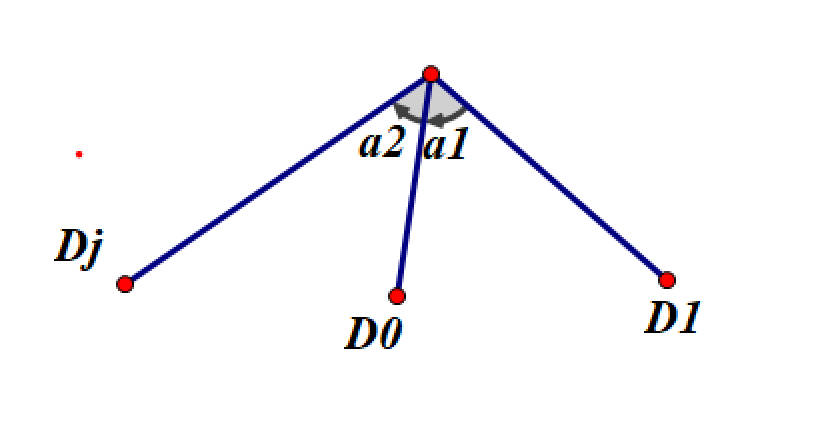
\includegraphics[width=0.4\linewidth]{../figures/1}}
			\subfloat[组态2]{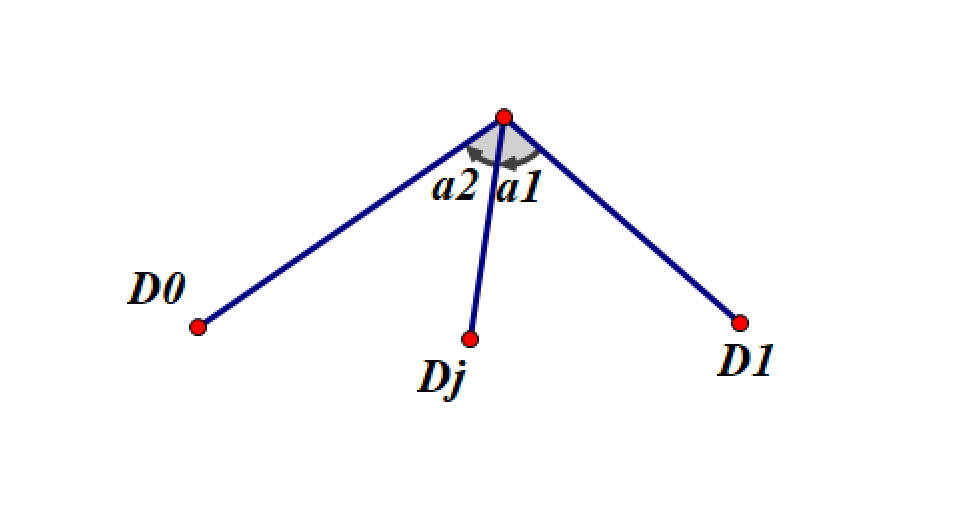
\includegraphics[width=0.4\linewidth]{../figures/2}}
			\caption{可能出现的两种组态}
			\label{fig1}
		\end{figure}
		基于以上公共知识,需要设计算法$D_i = f(\alpha_1, \alpha_2)$求解$D_i$在$D_0 - D_1$坐标系中的位置。
		\subsection{问题三:}
%----------- 三、模型的假设与约定 ----------
	\section{模型的假设与约定}
		\begin{itemize}
			\item{} one
			\item{} two
			\item{} three
		\end{itemize}
%----------- 四、符号说明及名词定义 ----------
	\section{符号说明及名词定义}
		\begin{center}
			\begin{table}[H]
				\caption{本论文所使用的符号}
				\begin{tabularx}{\textwidth}{p{0.08\textwidth}X}
					\toprule	
					$D_i$ & 编号为$i$的无人机的理想位置  \\
					$\widehat{D_i}$ & 编号为$i$的无人机的有偏实际位置  \\
					$D_i(\rho,\theta)$ & 用极坐标表示的无人机的位置 \\
					  
					$\overrightarrow{D_iD_k}$ & 从$D_i$指向$D_k$的矢量 \\
					$\omega_i$      & 编号为$i$的无人机的误差矢量,即$\overrightarrow{\widehat{D_i}D_i}$ \\
					$\bigodot O_i$    & 第$i$个理想圆  \\
					\bottomrule
				\end{tabularx}
			\end{table}

		\end{center}
%----------- 五、模型的建立与求解 ----------
	\section{模型的建立与求解}
		\subsection{问题一中第一问}
		\subsubsection{问题一中第一问模型的建立}
		\par 问题一首先限定了编队的飞机数目为10架并且编队方式为圆形编队,且要求其中一架无人机(编号为FY$ 00 $)位于圆心,而其余九架无人机位于相应的圆周上面。值得注意的是,无人机会基于自身感知的高度信息,均保持在同一个高度上飞行,因此我们可以将问题的求解模型确定在一个高度平面来方便求解下列各个问题。
		\par 
		而第一题的第一问则进一步明确无人机的角色:位于圆心的无人机(FY$ 00 $)和编队中另 $ 2 $ 架无人机发射信号,而其他无人机则是被动接受该三架无人机发射信号的角色。同时一个重要的条件是:模型要求在发射信号的无人机位置无偏差且编号已知的情况下完成其他被动接受信号的无人的定位。基于上述已知设定信息,我们可以首先将定位问题转换为二维平面上的位置求解问题。因为圆周的位置具有\textbf{高度对称性},因此不妨假设其中两台圆周上已知编号的信号发射无人机其中一台的编号为FY$ 01 $.因此我们可以在二维平面上选取编号为FY$ 00 $的无人机为原点,编号为FY$ 01 $的无人机为$ X $轴正方向的一点,从而建立笛卡尔右手坐标系如下图\ref{1-1}。
		\begin{figure}[htb]
			\centering
			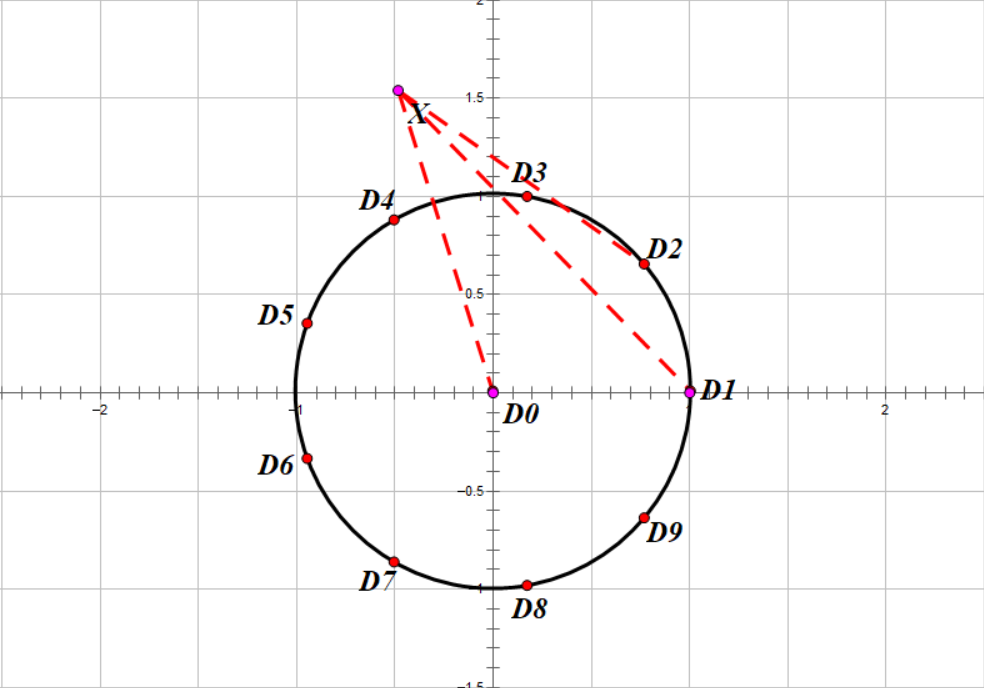
\includegraphics[width=0.7\linewidth]{./figures/Question1-1.png}
			\caption{问题一:定位模型坐标系}
			\label{1-1}
		\end{figure}
		在已知三架编号已知且位置无偏差的无人机后,我们可以在该坐标系中按直角坐标。同时对于编队中其他待定位的无人机,我们都可以得到与三架发射信号无人机的方位信息:任意两架发射信号无人机与待定位无人机的夹角。夹角代表着方向向量直接的位置关系,故应在表示待定位无人机的直角坐标后确定发射信号的无人机与待定位无人机连线的方向向量,进而再表示出夹角然后求解。
		\subsubsection{问题一中第一问的具体求解}
		\par 基于第一问的定位模型,我们建立以已知编号FY$ 00 $ 的无人机为原点$ D_0 $ ,而另外两架已知编号的$ \text{无人机}i\text{与无人机}j $ $ \text{无人机}i\text{与无人机}j $ 分别设为$ D_i\text{与}D_j $ ,其极坐标对应的为$ \left( r,\beta _i \right) ,\left( r,\beta _j \right)  $ ,其中$ \beta _i\text{与}\beta _j $ 均可通过编号得到,为已知数据。不失一般性,我们将其他所有待定位的无人机$ X $ 的极坐标设为$ \left( \rho ,\theta \right)  $ 。根据题意我们可知无人机$ X $ 会接收到位于设定原点的无人机$ 00 $ 和$ \text{无人机}i\text{与无人机}j $ 发射的电磁信号,进而可以提取的信号为:该无人机$ X $ 与任意两架发射信号的$ \text{无人机}i\text{与无人机}j $ 连线之间的夹角,即$ \left( \begin{array}{c} 	3\\ 	2\\ \end{array} \right)  $ 共三个角度的方位信息。根据几何知识,可以得到该三个角中最大的角为其余两个角的和。因此,为减少信息的冗余性,我们只利用其中两个角:$$ \alpha _i=\angle OXi\text{,}\alpha _j=\angle OXj $$ 
		\par 至此,我们从极坐标转至直角坐标系: 
		$$ D_0\text{:}\left( 0,0 \right)  $$ $$ D_i\text{:}\left( r\cos \beta _i,r\sin \beta _i \right)  $$ $$ D_j\text{:}\left( r\cos \beta _j,r\sin \beta _j \right)  $$ $$ D_X\text{:}\left( \rho \cos \theta ,\rho \sin \theta \right)  $$ 
		\par 因此可以进而得到三个向量:
		$$ \overrightarrow{D_0D_X}=\left( \rho \cos \theta ,\rho \sin \theta \right)  $$ $$ \overrightarrow{D_iD_X}=\left( \rho \cos \theta -r\cos \beta _i,\rho \sin \theta -r\sin \beta _i \right)  $$ $$ \overrightarrow{D_jD_X}=\left( \rho \cos \theta -r\cos \beta _j,\rho \sin \theta -r\sin \beta _j \right)  $$ 	
		\par 紧接着,我们通过三个向量分别利用余弦定理,分别表示出$ \alpha _i\text{与}\alpha _j $: 
		$$ \cos \alpha _k=\frac{\rho ^2\sin ^2\theta -r\rho \cos \beta _k\cos \theta +\rho ^2\cos ^2\theta -r\rho \sin \beta _k\sin \theta}{\rho ·\sqrt{\rho ^2\sin ^2\theta +r^2\sin ^2\beta _k-2r\rho \sin \beta _k\sin \theta +\rho ^2\cos ^2\theta +r^2\cos ^2\beta _k-2r\rho \cos \beta _k\cos \theta}} $$ $$ \text{即:}\cos \alpha _k=\frac{\rho -r\cos \left( \theta -\beta _k \right)}{\sqrt{\rho ^2+r^2-2\rho r\cos \left( \theta -\beta _k \right)}}\ \ \ \ \ \left( k=i,j \right)  $$ 
		\par 由此求解 两个方程:$ \text{通过}\frac{\rho}{r}\text{和}\theta \text{表示的}D_X\text{具体坐标} $ 从而完成定位。
			
		\subsection{问题二}
			经过我们的研究,我们认为需要除了在圆心的0号,还需要在圆弧上的1号和另外一个j号共三架飞机发射信号才能确定任意一架飞机i的位置。我们的位置解算算法遵循机组组态分析、推断匿名第三者编号、可行域分割的步骤求出$D_i$的坐标。在使用逐步分割可行域的方式求解位置坐标时,我们针对多解的情况,着重讨论了对于“略有偏差”的数学定义。
			\subsubsection{算法的求解过程分析}
			对于问题$D_i = f(\alpha_1, \alpha_2)$,我们首先需要确定第三架飞机是标签为几的飞机。以待测飞机为2号机,匿名第三信号发射机为3号机为例,建立数学几何模型。
			\paragraph{机组组态分析}
			待测飞机为2号机的情况下,2号机接收到的三个角度值遵循$\angle D_jD_2D_1 =\angle D_jD_2D_0 + \angle D_jD_2D_1$,符合\ref{fig1}中所示组态1的类型。
			\paragraph{匿名第三者位置分析}
			在组态1的情况下,匿名第三者编号$j=3,4,5,6$中的一个。
			\paragraph{可行域分割}
			对于所有可能的$D_j$,现已确定$\angle D_jD_2D_0 = \alpha_1$,$|D_jD_0|= r$,对于此类定弦定角问题,有优弧$\overset{\frown}{D_jD_2D_0}$上的点为所有可能的$D_2$的位置。
			对于确定的$\angle D_0D_2D_1 = \alpha_2$,$|D_1D_0|= r$优弧$\overset{\frown}{D_0D_2D_1}$上的所有点为所有可能的的$D_2$的位置。
			\begin{figure}[htb]
				\centering
				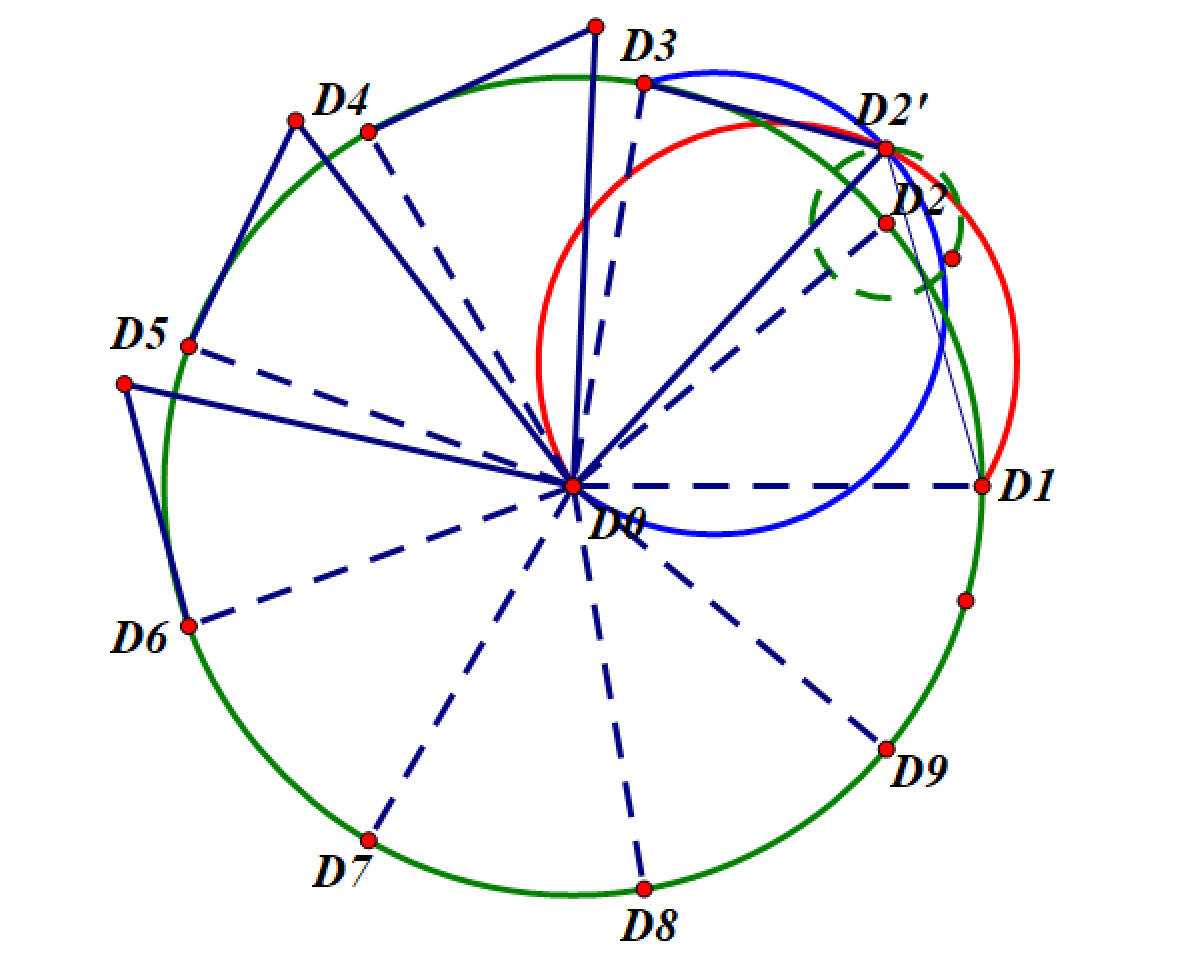
\includegraphics[width=0.5\linewidth]{./figures/3}
				\caption{$\angle D_3D_2D_0$ 的可行域$\overset{\frown}{D_3D_2D_0}$与$\angle D_0D_2D_1$ 的可行域$\overset{\frown}{D_0D_2D_1}$}
				\label{fig3}
			\end{figure}
		
		
			如图\ref{fig3}所示,对于有微小偏差的无人机$D_2'$,当假设匿名第三者为无人机3时,有可能位置$P$。同理,分别建立匿名第三者$j=4,5,6$时,$D_2'$的可能位置,分别标记为$Q,R,S$,如图\ref{fig4}.
			
			\begin{figure}[htb]
				\centering
				\subfloat[所有可能可行域集合]{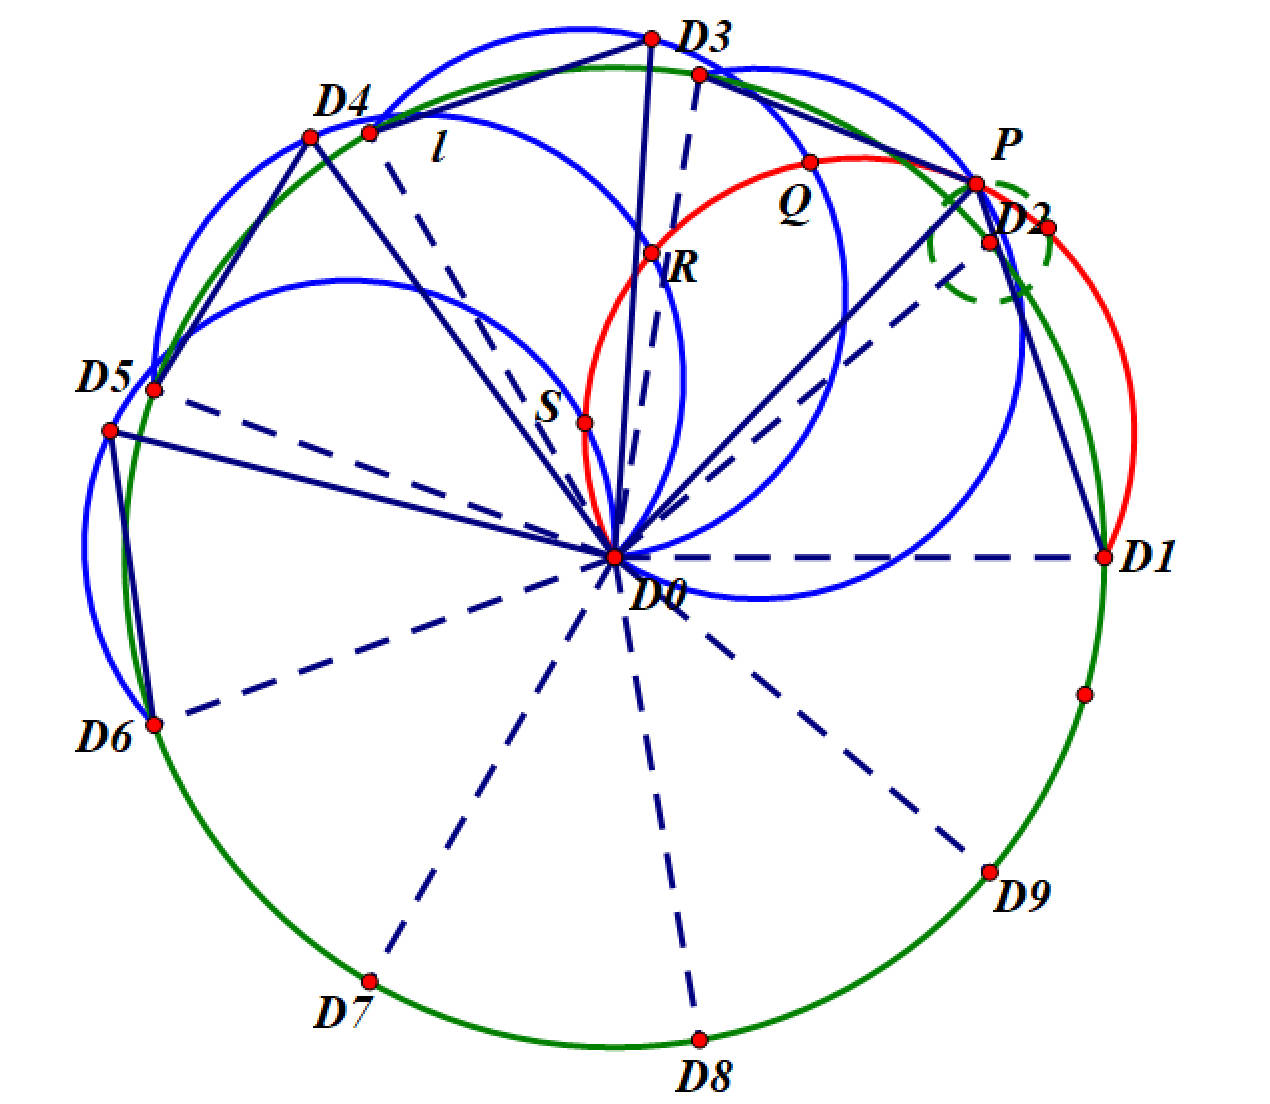
\includegraphics[width=0.4\linewidth]{../figures/4}}
				\subfloat[$D_2'$的可能位置$P,Q,R$]{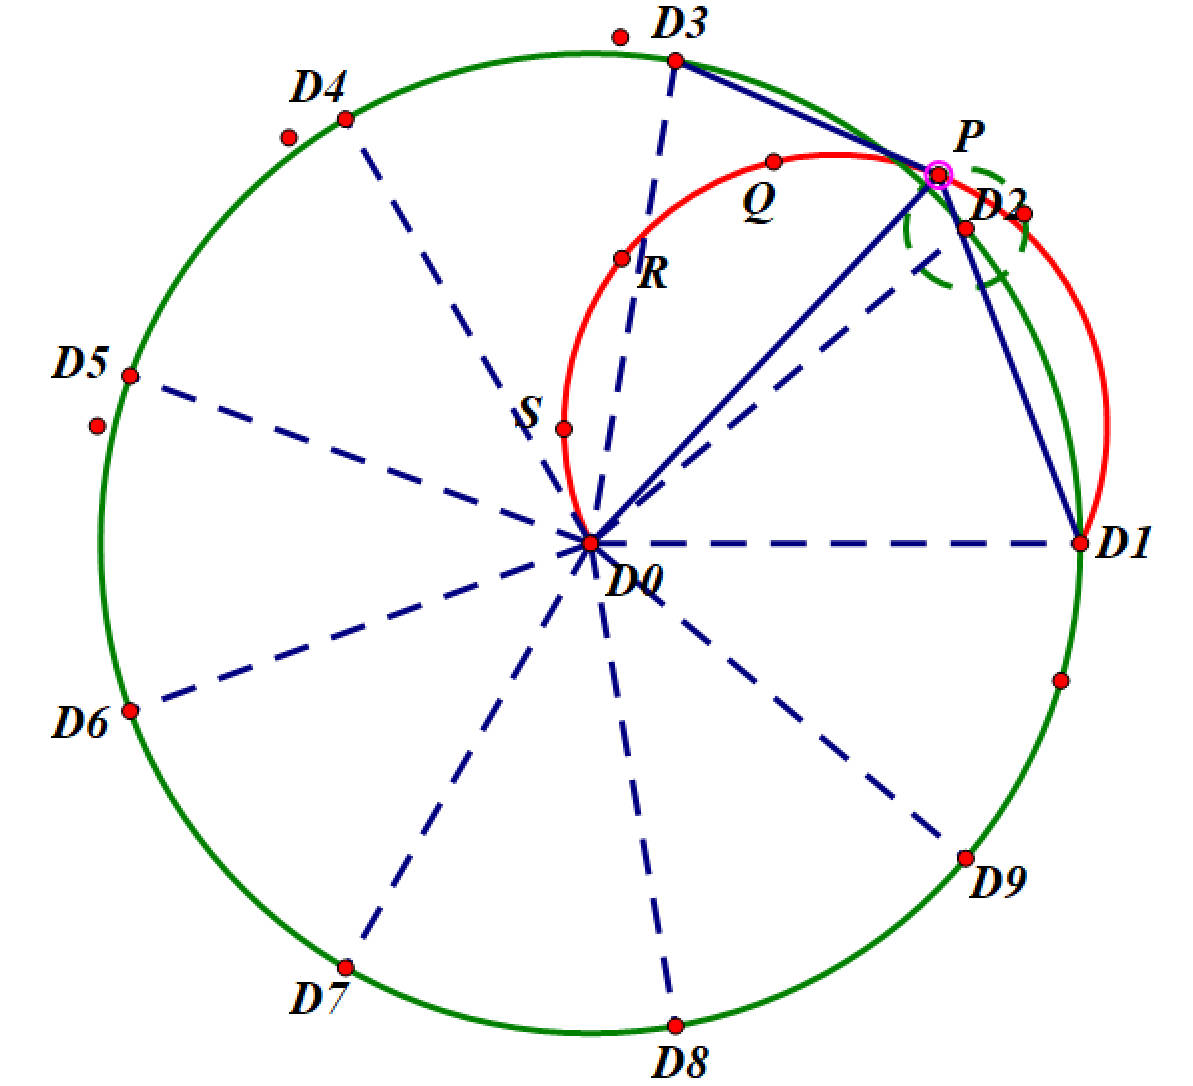
\includegraphics[width=0.4\linewidth]{../figures/5}}
				\caption{$D_2'$的可能位置的求解}
				\label{fig4}
			\end{figure}
			
			至此,对于不确定匿名第三者的情形,飞机$D_i$($D_2$)由于不能确定第三者编号产生了自己的位置猜测$P,Q,R,S$,在图\ref{fig4}的情形下,易确定$R,S$的情形不符合题设从而排除,然而我们观察到当2号机偏差很大时(即$\lVert\omega_i\rVert =\overrightarrow{D_2D_2'} $很大时)有可能出现情形如图\ref{fig6}.此时若认为第三者为4号机,则会有位置错误估计Q,然而在此种情形下,我们认为其实际位置应为图中P点的位置。因为此种情况的出现,我们要对“偏差较小”进行数学定义。
			\begin{figure}[htb]
				\centering
				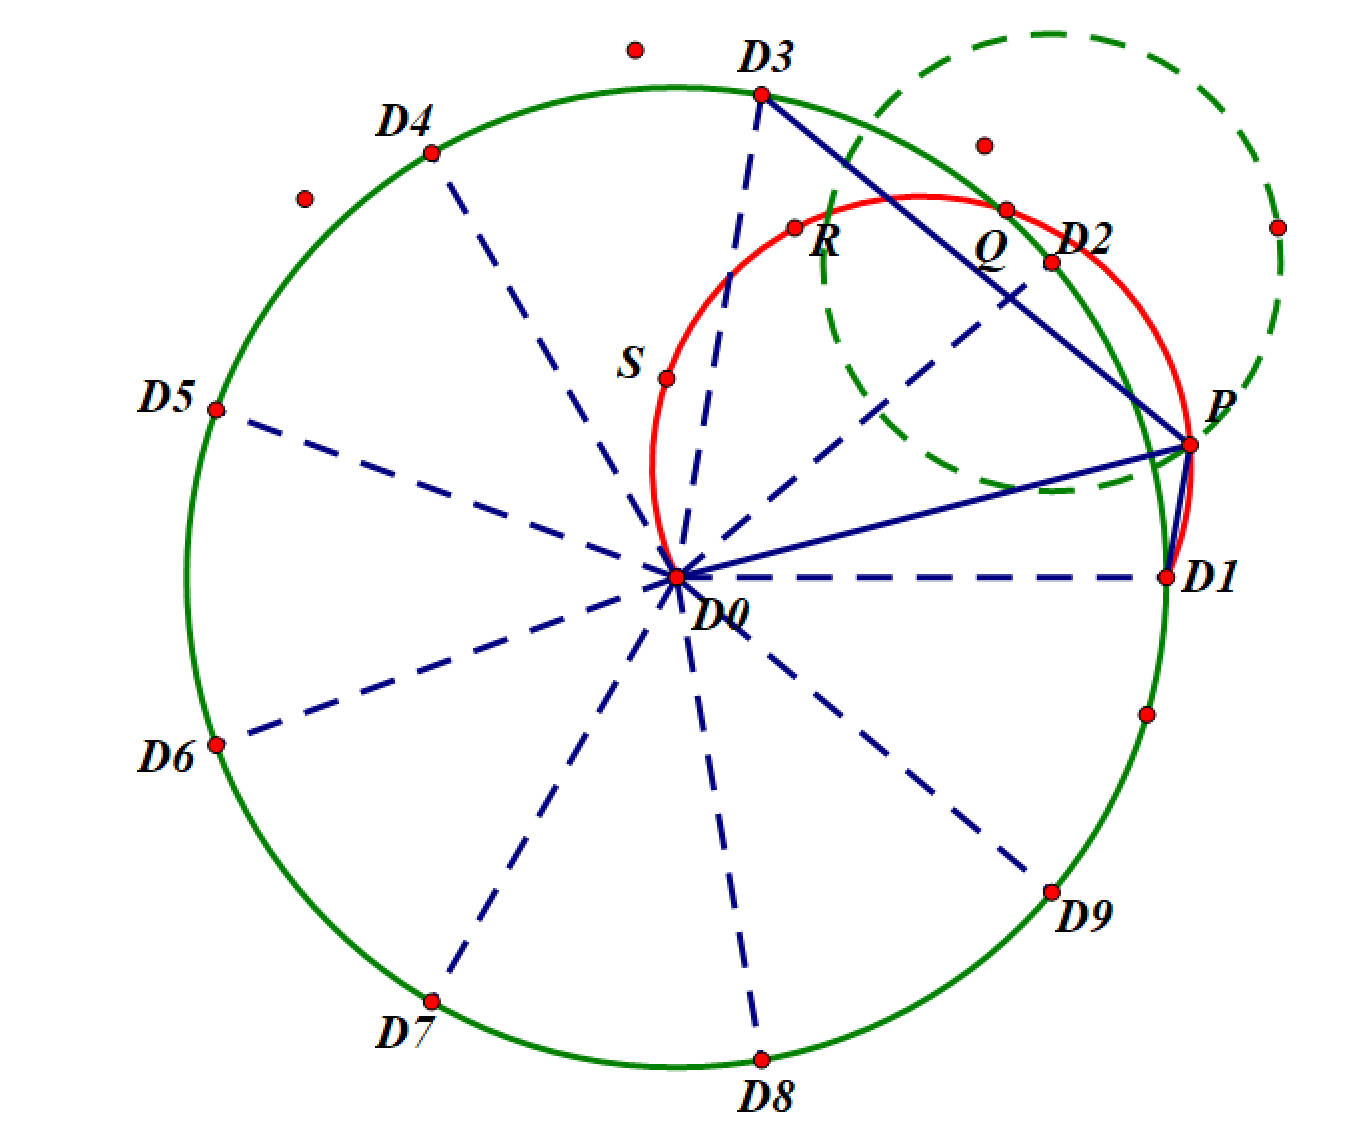
\includegraphics[width=0.5\linewidth]{./figures/6}
				\caption{偏差很大时的一种特殊情况}
				\label{fig6}
			\end{figure}
		
		
			\paragraph{多解分析}
			因为在三架飞机定位的模式下,匿名第三者未知。这种情况下待定位飞机对于自己的位置估计就可能出现多解的情况。然而我们发现,在待定位飞机距离无偏差位置很远的时候,不能通过解的合理性排除多解情况。所以我们进一步探索了多解的可排除情况的边界条件。
			
			
			当$ D_2' $ 运动在区域:$ \lVert \omega _2 \rVert \le r_0 $ 内时,$ \text{运动点}P\text{、}Q\text{、}R\text{、}S\text{的集合分别记为}\mathcal{P}\text{、}\mathcal{Q}\text{、}\mathcal{R}\text{、}\mathcal{S} $ 建立动态几何解析模型,使$ D_2' $在其运动区域边界上运动时,跟踪$P,Q,R,S$的轨迹,其内部即为$\mathcal{P}\text{、}\mathcal{Q}\text{、}\mathcal{R}\text{、}\mathcal{S}$.
			
			\begin{figure}[H]
				\centering
				\subfloat[$r_0$很小时的运动轨迹情况]{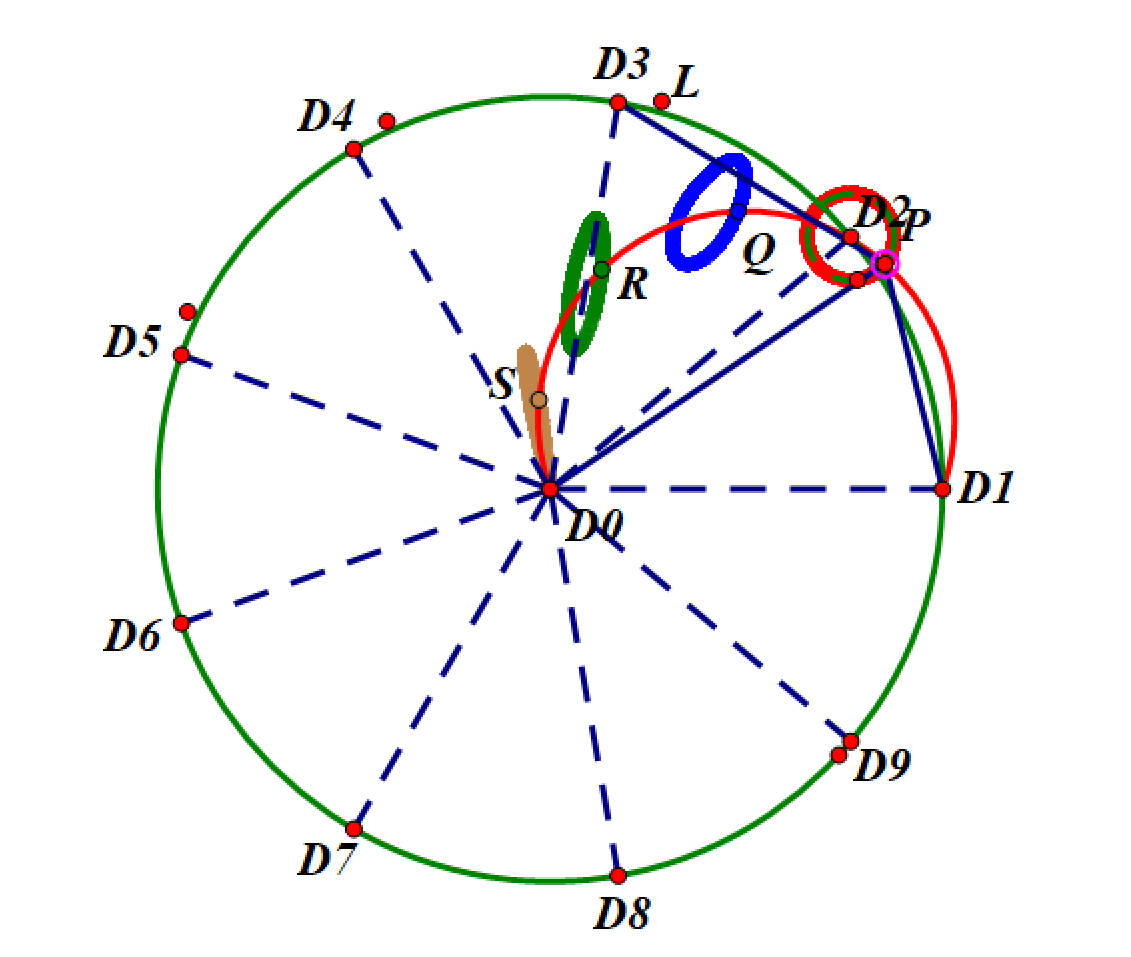
\includegraphics[width=0.43\linewidth]{../figures/7}}
				\subfloat[$r_0$处于临界时的运动轨迹情况]{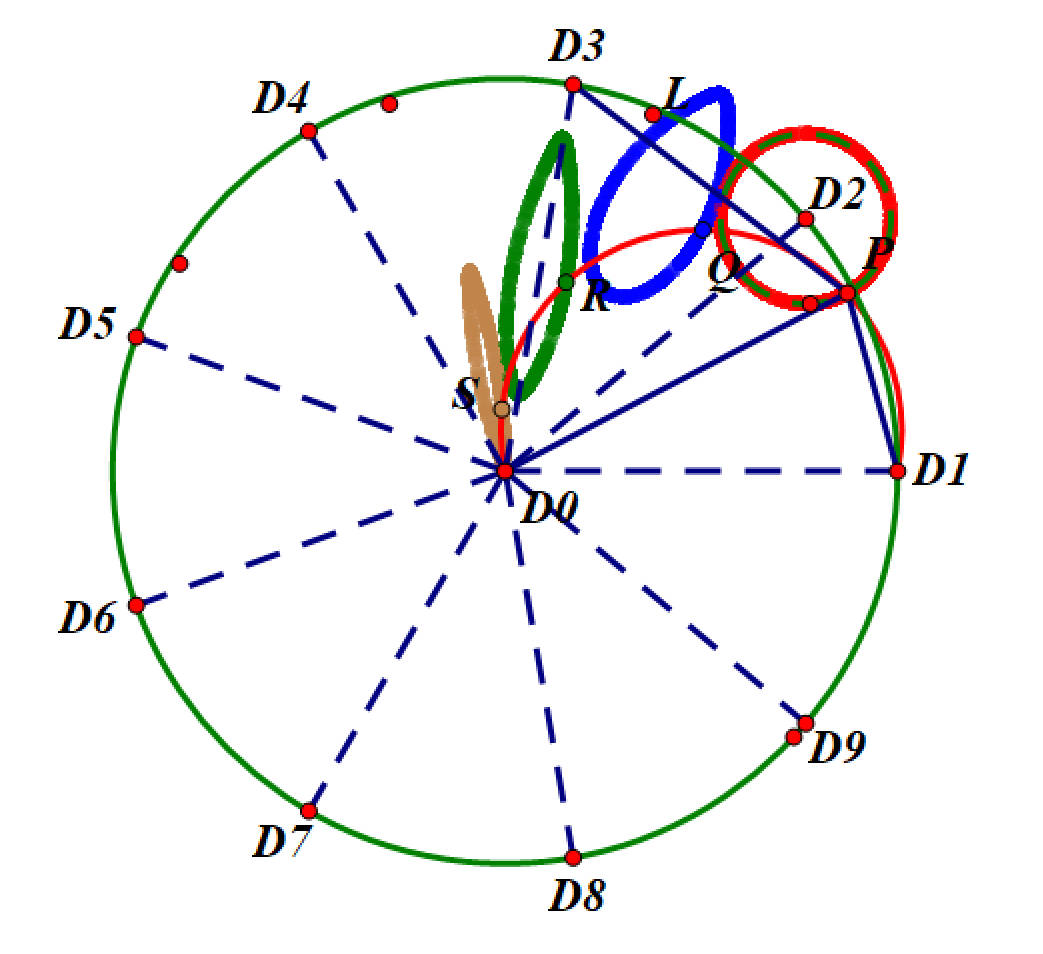
\includegraphics[width=0.4\linewidth]{../figures/8}}
				\\
				\subfloat[$r_0$很大时的运动轨迹情况]{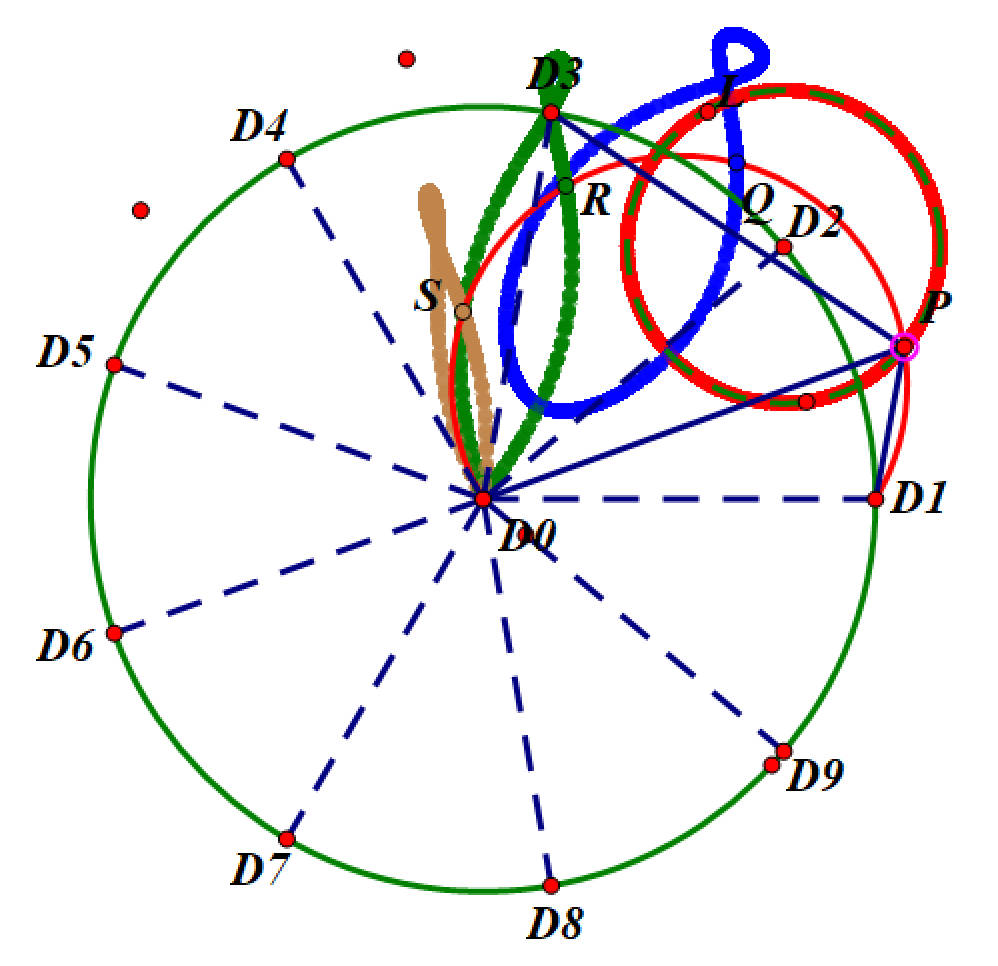
\includegraphics[width=0.4\linewidth]{../figures/9}}
				\caption{不同$r_0$的取值下$\mathcal{P}\text{、}\mathcal{Q}\text{、}\mathcal{R}\text{、}\mathcal{S}$的边界分布}
				\label{fig7}
			\end{figure}
			从图\ref{fig7}可以看出,$r_0$很大时,$\mathcal{P}\text{、}\mathcal{Q}$的边界有重叠,即$
			\exists p\in \mathcal{P},\ q\in \mathcal{Q}\ \ s.t.\ \left| \overrightarrow{pD_2} \right|\ >\left| \overrightarrow{qD_2} \right|$ 此时根据如果根据预测点到理想点最近的原则确定匿名无人机编号,将会误认为是$D_4$发射的信号,进而将自己的位置误认为$q$的位置。如图\ref{fig4}所示,此时无人机的实际位置为P但是根据上述算法会将其误认为Q。
			
			使用动态几何求解器,我们求得在上述情形下$\mathcal{P}\text{、}\mathcal{Q}$边界相切时,$r_{2max}\approx 0.228\left| \overrightarrow{D_0D_1} \right|$。
			进一步,我们探索了匿名无人机变化与边界情况$r_0$的最大取值之间的关系。我们得出结论:$r_0$的最大取值与匿名无人机的的变化无关,只与待测无人机的编号有关。
			\begin{figure}[H]
				\centering
				\subfloat[匿名无人机为$D_3$时的边界情况]{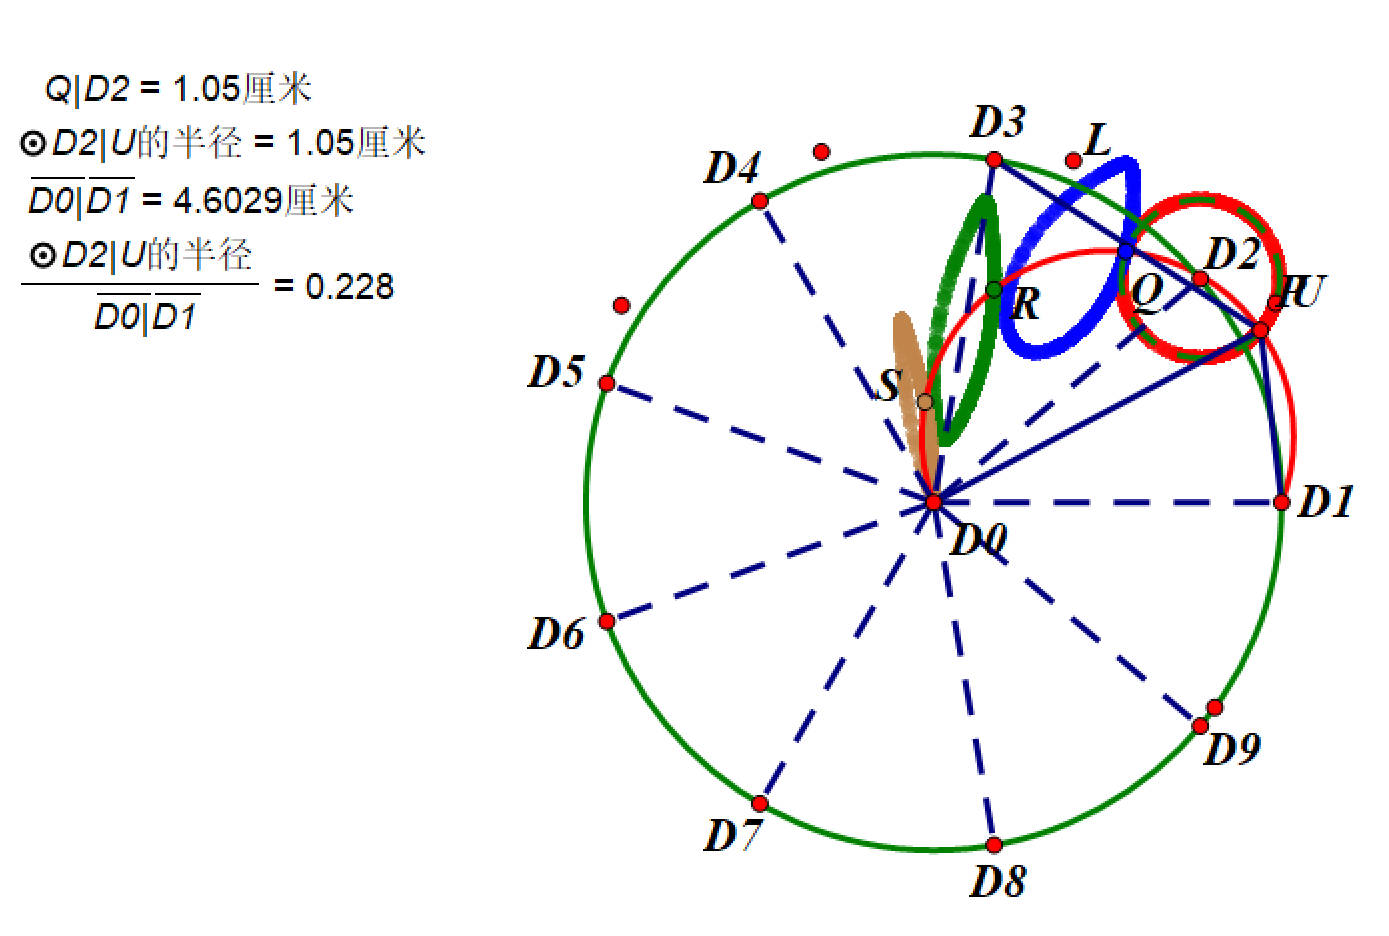
\includegraphics[width=0.45\linewidth]{../figures/10}}
				\subfloat[匿名无人机为$D_4$时的边界情况]{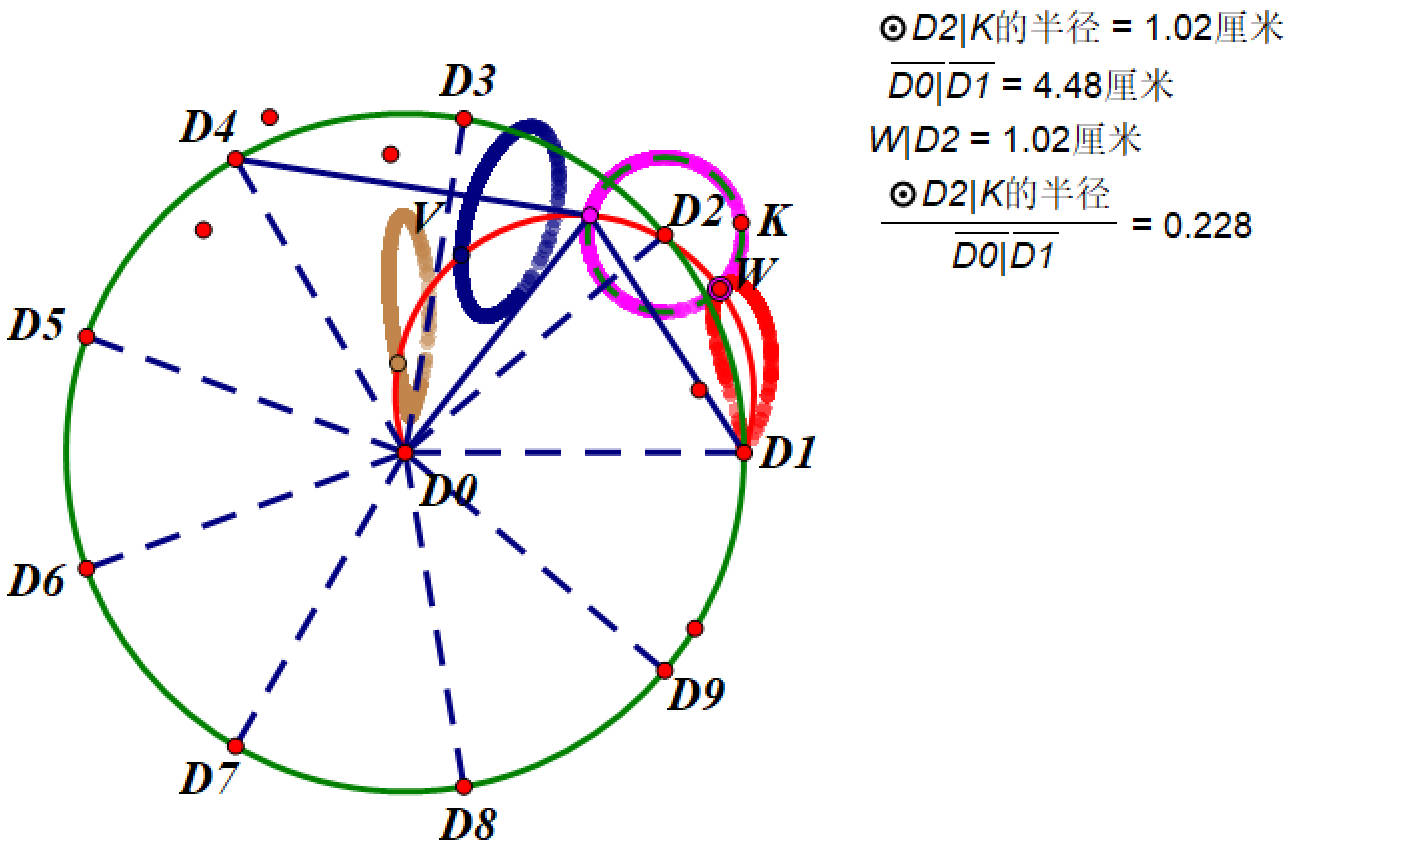
\includegraphics[width=0.45\linewidth]{../figures/11}}
				\caption{不同匿名无人机情况对于$D_2$唯一解边界情况的影响}
				\label{fig10}
			\end{figure}
		
			进一步,我们探索了不同待测无人机的最大误差范围。
			根据我们的模拟,我们有如下临界情况:
			\begin{figure}[H]
				\centering
				\subfloat[待测无人机为$D_3$时的边界情况]{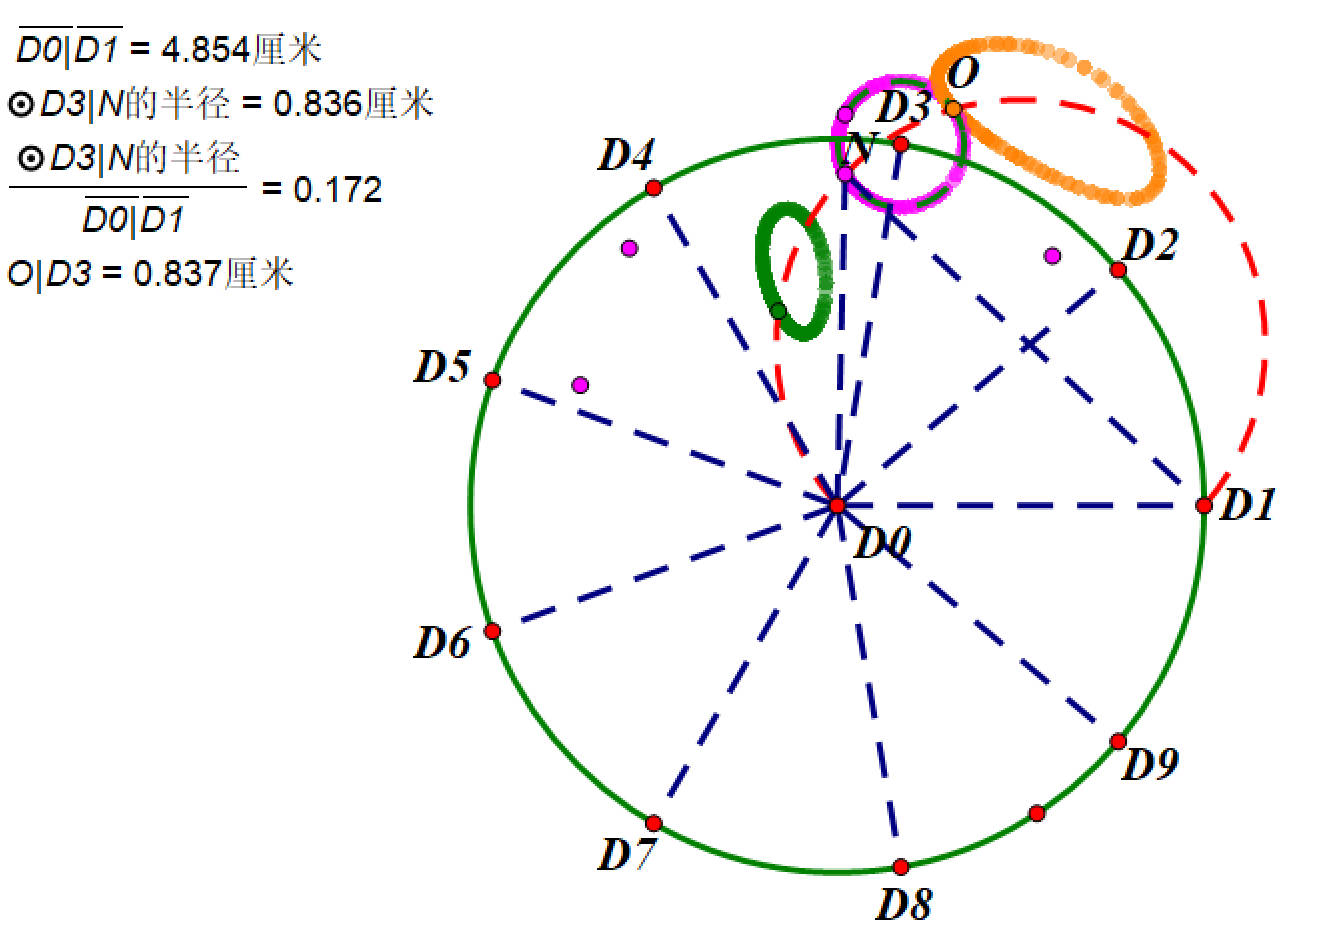
\includegraphics[width=0.45\linewidth]{../figures/12}}
				\subfloat[待测无人机为$D_4$时的边界情况]{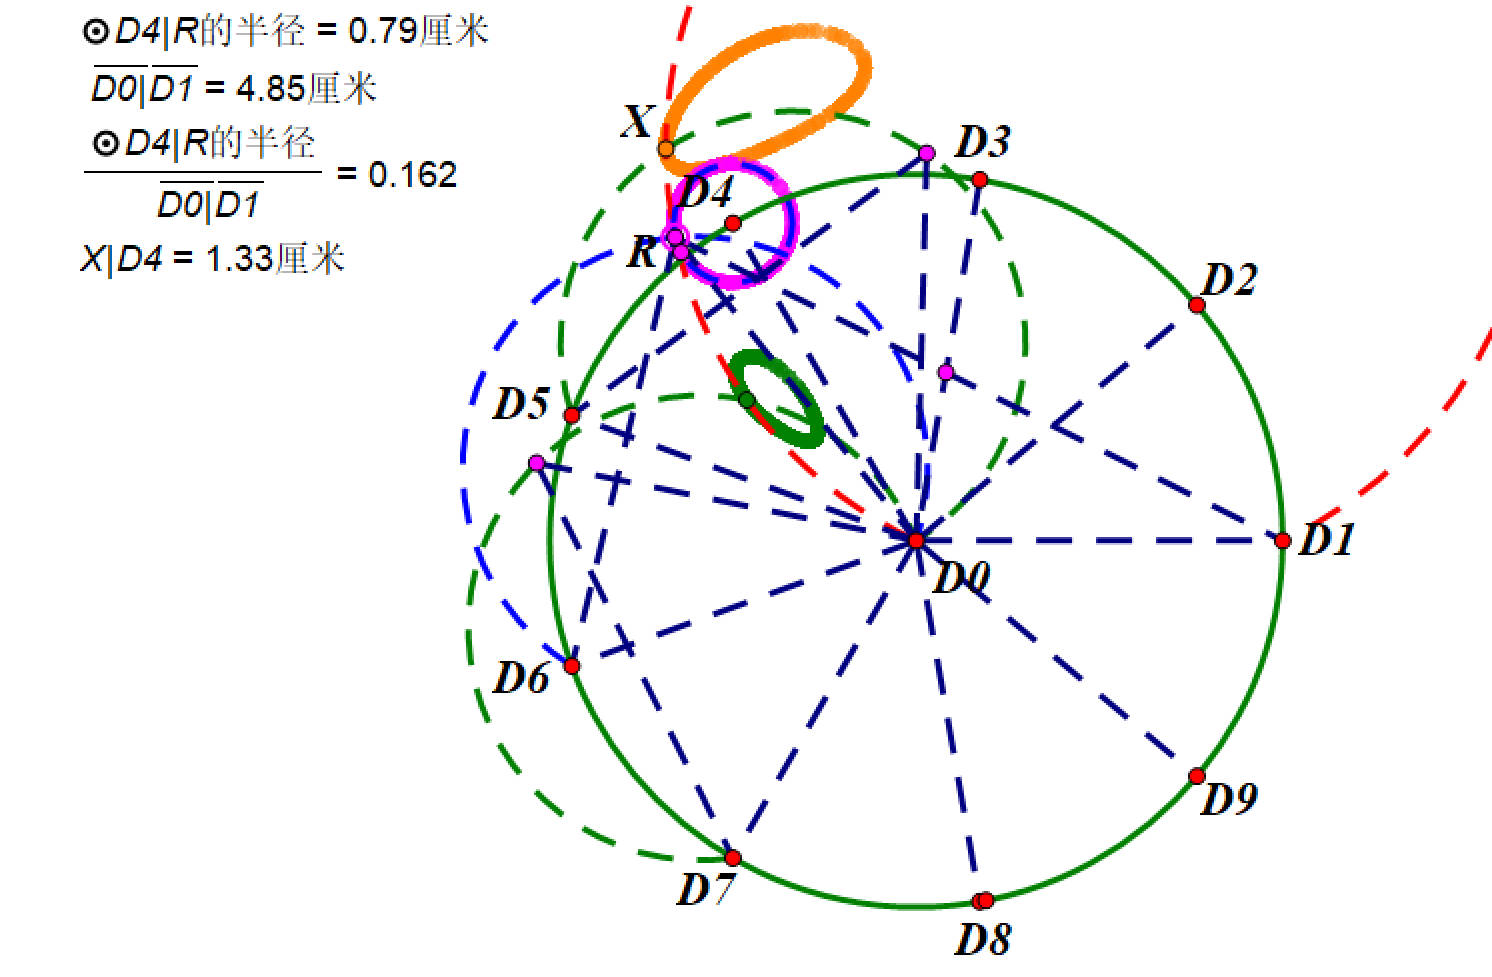
\includegraphics[width=0.45\linewidth]{../figures/13}}
				\\
				\subfloat[待测无人机为$D_5$时的边界情况]{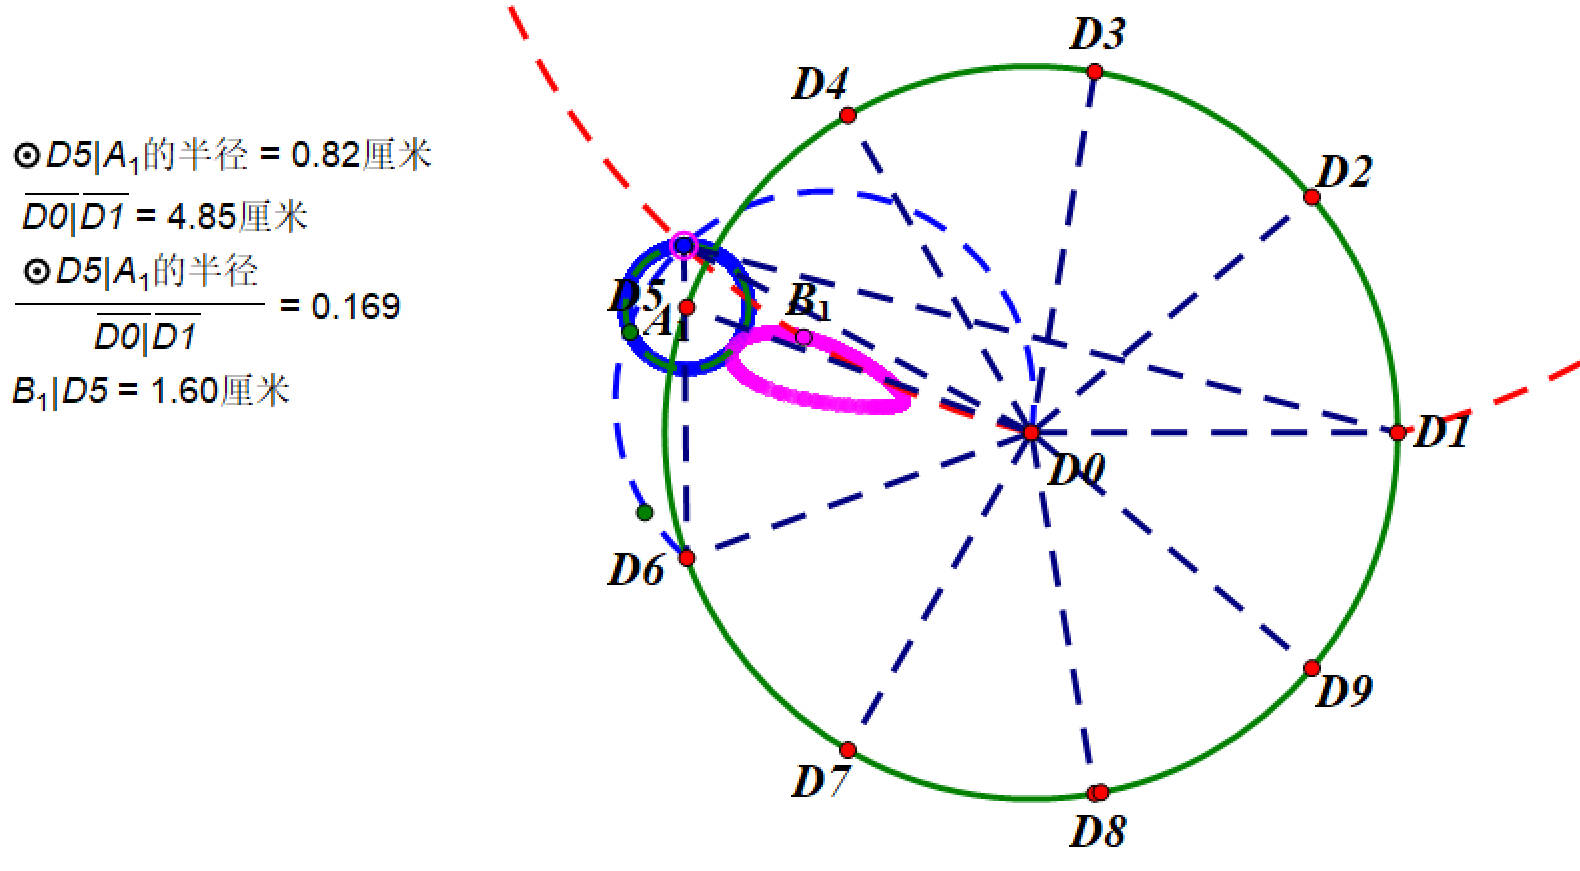
\includegraphics[width=0.5\linewidth]{../figures/14}}
				\caption{不同待测无人机唯一解边界情况}
				\label{fig12}
			\end{figure}
			令$r_i$为第i个无人机作为待测无人机时,有单一解时$\overrightarrow{\widehat{D_i}D_i}$的模长。
			我们分别得出,$r_{3max}\approx 0.172\left| \overrightarrow{D_0D_1} \right|,r_{4max}\approx 0.162\left| \overrightarrow{D_0D_1} \right|,r_{5max}\approx 0.169\left| \overrightarrow{D_0D_1} \right|$。
			根据对称性,我们同理可得$D_6,D_7,D_8,D_9$分别为待测无人机的情况。
			
			综上,我们进而给出对于任意的无人机,其“偏差较小”的数学定义为$|\overrightarrow{\widehat{D_i}D_i|}<0.162|\overrightarrow{\widehat{D_0}D_1}|$。若知道具体编号,则可以适用不同的边界情况数据。
			\subsubsection{title}
			\subsubsection{title}
		\subsection{问题三}
			\subsubsection{title}
			\subsubsection{title}
			\subsubsection{title}
	\section{总结}
	\begin{thebibliography}{9}%宽度9
		\bibitem{bib:one} ....
	\end{thebibliography}
	\begin{appendices}
		附录的内容。
	\end{appendices}
\end{document}